\chapter{Running Example}
\label{running-example}

For our running example, we use a modified scenario based on a real-life problem, which
was first introduced in \citep{isola2018}. We will refer back to this scenario
throughout the work, in order to showcase problems, features of the DSL, and
implementation details.

\section{Scenario}

The scenario models a company that works on sensitive projects for its clients. At any
given time, multiple projects can be developed in parallel. Developers working on the
same project must be able to cooperate. However, to limit exposure of sensitive
intellectual property, developers from different projects should not come into contact
with each other; namely, developers of two different projects are not allowed to stay in
the same room while in the company building. To this end, each developer has a smart
device (mobile phone, smart watch, etc.) that can direct them to the appropriate rooms.

We assume that each developer is assigned to exactly one project. Only two types of
rooms are considered: workrooms and lunchrooms.

Workrooms are open whenever the building is open, which is from 7:30~AM to 9~PM. Each
workroom is assigned to a particular project. All developers on a project are permitted
to enter all workrooms for that project, to allow for efficient collaboration. We assume
that workroom assignment is fixed for the duration of our scenario and that it provides
enough capacity for all developers of a given project.

Lunchrooms only open around midday, from 11:30~AM to 3~PM. Each lunchroom has a set
maximum occupancy. We expect that there will not be enough lunchrooms to seat all
developers, esp. with the constraint that developers from different projects must not
meet in the same room. Therefore, room assignment must be dynamic. Developers will be
equipped with smart devices which can send seating requests and display the current
situation.

\medskip

Our interest lies in access permissions. Specifically, we want to investigate which
developers can enter which rooms at various times and under various conditions, and how
an access control system could handle a given situation.

\begin{figure}[t]
    \centering
    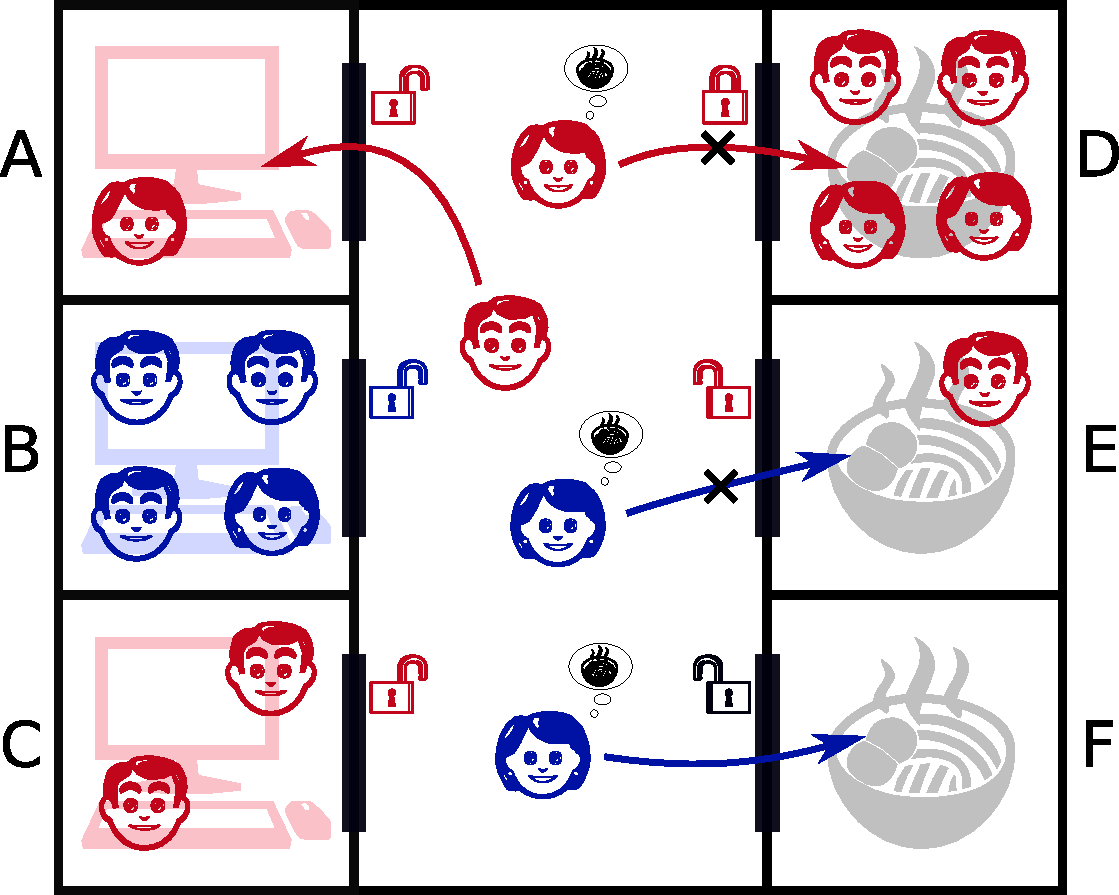
\includegraphics[width=1\linewidth]{img/lunch-rules.pdf}
    \caption{Example scenario with workrooms and lunchrooms}
    \label{fig:lunch-rules}
\end{figure}

Figure~\ref{fig:lunch-rules} illustrates a possible situation. Developers on blue and
red projects are moving around in the building, which has three lunchrooms and three
workrooms. Two workrooms (computer symbol) are assigned to the red project and one is
assigned to the blue project, as indicated by the symbol color. Lunchrooms (food symbol)
are not assigned to projects. Each room has a capacity of four people.

There is a red, blue or black lock on each door. Red and blue indicates that the door is
open to developers of the corresponding project. Black indicates that anyone can open
the door. The lock on room D is closed, showing that nobody can enter. In this case, it
is because the room is full.

Room B is also full, but the lock remains open, because our security policy does not
take workroom capacity into account.

The red worker in the middle is allowed to enter room A, because it is a workroom
assigned to a red project. The hungry red worker is not allowed to enter room D,
however, because the room is full. She would be allowed to enter room E, currently open
to developers of red project, but the hungry blue worker in the middle cannot do that.
There is already a red worker inside, and the security policy disallows developers from
different projects to meet in the same room. Hungry blue worker at the bottom can enter
room F, because it is empty, so no security conflict arises.

\section{Workroom Assignment}

If we ignore lunchrooms for a moment, the problem is relatively simple. Access
permissions are known in advance. At night, no rooms are open and nobody is allowed to
enter. In the day, every developer assigned to a particular project is allowed to enter
every workroom assigned to that same project. We can enumerate the available workrooms,
and for each one, enumerate all persons allowed to enter that room. Only those people
are allowed to enter, and no other access permissions exist. The rules are fixed and
don't need to be updated except when scenario definition changes.

\begin{figure}[ht]
    \centering
    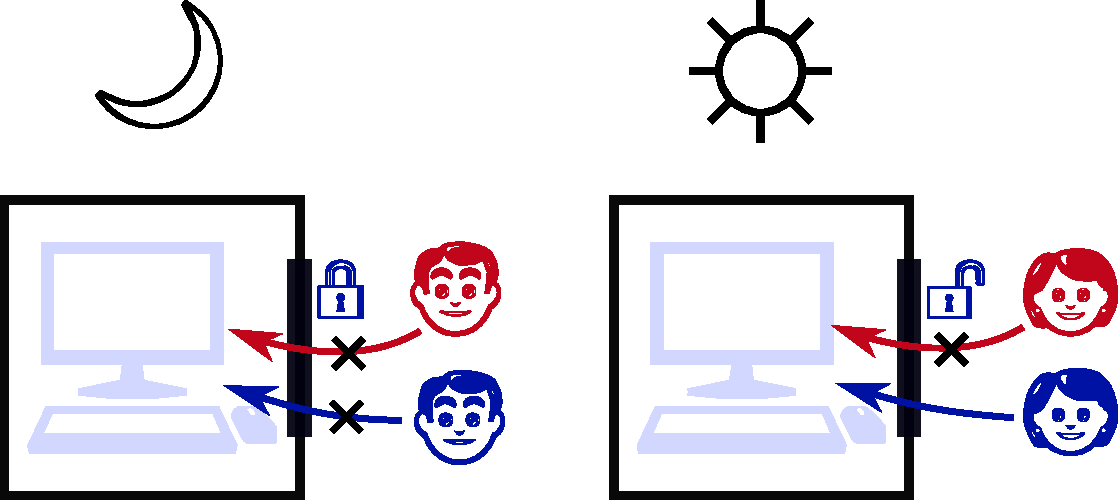
\includegraphics[width=1\linewidth]{img/workroom-access.pdf}
    \caption{Workrooms at night and in the day}
    \label{fig:workroom-access}
\end{figure}

Figure~\ref{fig:workroom-access} shows all possible configurations. Either it is night
time, in which case nobody can enter, or it is daytime, and blue developers can enter,
while red ones cannot. This scenario is easy to solve even in traditional entity-based
access control systems. The only dynamic parameter is time of day, which is commonly
supported on contemporary electronic locks.

\section{Lunchroom Assignment}

During lunch hours, a developer can request seating in a lunchroom. This introduces a
dynamic and unpredictable element. It is no longer sufficient to \textit{enforce} access
control rules, we need to re-evaluate the situation and generate new access grants.

\medskip

There are several possible approaches to this situation. One option is to leave the
choice to the human: during lunch hours, every developer is allowed to enter every
lunchroom, except when (a) the lunchroom is full, or (b) developers from a different
project are already present in the lunchroom. The advantage of this approach is twofold.
First of all, it gives greater freedom to the developers. The system is not trying to
make decisions for them, and everyone can choose a lunchroom based on their own
criteria, such as how close it is, where their friends sit, etc. Second, because the
system does not need to make choices, it is computationally simpler. We need to monitor
the situation and update access grants based on current seating and room capacity, but
we can still describe the situation using conditional entity-based rules.

There are some drawbacks, too. When individual developers choose lunchrooms for
themselves, they only take their local context into account. This can lead to a
situation shown on figure~\ref{fig:lunch-inefficient}. Red developers have occupied
all the available lunchrooms. Even though there is more than enough total available
seats, none of the hungry blue developers can use them.

There is also no way to reserve a seat in advance; a developer could head out towards
their favorite lunchroom, only to find out that it is occupied and they need to go
elsewhere.

\begin{figure}[ht]
    \centering
    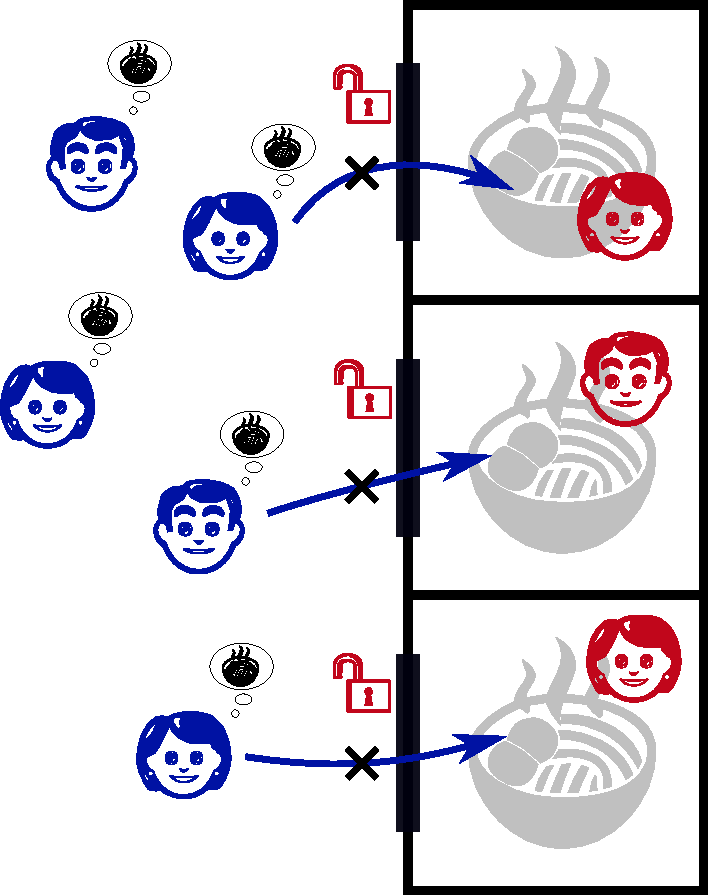
\includegraphics[width=0.67\linewidth]{img/lunch-inefficient.pdf}
    \caption{Inefficient use of available lunchrooms}
    \label{fig:lunch-inefficient}
\end{figure}

\medskip

On the opposite end of the spectrum, we can have the access control system make all the
decisions. We are working with the assumption that developers are free to choose
\textit{when} they want lunch, so we cannot simply pre-generate fixed time slots and
seats and solve a scheduling problem. However, we can still assign a particular
lunchroom whenever a developer requests a seat. The rule would be as follows: during
lunch hours, a developer can request a lunchroom. When a valid seat becomes available,
the developer is allowed to enter the assigned lunchroom once. When they leave the
lunchroom, their seat is freed for next requests.

This is the variant that we will be using in the rest of this work. It gives us the
opportunity to explore behavior of an access control system with regards to solving
conflicting and/or overlapping requirements.

\medskip

We must note, however, that in the real world, a less strict system would be preferable.
Perhaps a hybrid of the two outlined here: allow the developers to choose a lunchroom
based on individual preferences, reserve a seat through a smart device, while employing
heuristics to keep some free lunchrooms so that no project is starved, both in the
technical and the literal sense.

\section{Assignment Criteria}

When assigning lunchrooms, we must satisfy the scenario rules: developers from
different project must not be allowed to enter the same room, and we cannot assign
more developers to a lunchroom than its capacity. But in addition, we might want to
optimize for other criteria.

First of all, we want to achieve good utilization and availability of lunchrooms. More
specifically, every lunch request should be serviced as soon as possible, and thus every
developer should be able to have lunch at the time of their choosing. This means two
things: (1) we need to seat as many developers as possible at the same time, and (2) at
any given time, we should be able to seat a developer from any project.

While obviously limited by total capacity, there is a lot of room for different choices
with regard to these criteria. Consider a situation where a group of 6 developers from
project $A$ and a group of 4 developers from project $B$ request lunch simultaneously,
and there is only one free lunchroom available. By (1), we should seat the group from
project $A$, because it is bigger. But if all the other lunchrooms are occupied by
project $A$, we should probably give the room to the $B$ group to better achieve (2) ---
this would reserve the free space for more developers of project $B$, while we can
expect spaces for $A$ developers to become available in the other lunchrooms.

\medskip

We could continue adding criteria, of course. Earlier requests should have priority. It
might be desirable to assign lunchrooms that are physically close to the requester. We
might try to keep groups together. Perhaps requests should be prioritized by employee
seniority, or maybe we should even keep reserved seats for the bosses at all times. Each
developer could sort the lunchrooms by preference and their selection should be taken
into account.

Obviously, each additional criterion is making the problem more complex. It is not our
goal to solve this complexity; the point here is to show that requirements can vary and
this needs to be taken into consideration.
